\documentclass[a4paper,10pt]{report}\input{../0.Préambule/Préambule_cours_prof}\begin{document}

\pagestyle{empty}
\newpage
\section*{\hspace{11cm}Pyramide et cône}
\addcontentsline{toc}{section}{Pyramide et cône}

\medskip
\noindent
\hspace{11cm}\textbf{Exercice 1}: \hfill \textbf{5 points}

\vspace{-4cm}
\begin{tikzpicture}[line cap=round,line join=round,>=triangle 45,x=1.0cm,y=1.0cm]
\clip(-0.1,-27.) rectangle (16.,0.1);
\draw [shift={(2.8044542158722416,-20.60614809830412)},line width=2.pt,color=red,fill=red,fill opacity=0.1] (0,0) -- (-28.11785716868146:1.2505519579210644) arc (-28.11785716868146:85.88214283131855:1.2505519579210644) -- cycle;
\draw [line width=2.pt] (4.,-4.) circle (4.cm);
\draw (1.5696807125702315,-5.406497289701779) node[anchor=north west] {OM = 4};
\draw (-0.05603683272715222,-13.95193566882904) node[anchor=north west] {MS = 12.65};
\draw [shift={(2.8044542158722416,-20.60614809830412)},line width=2.pt]  plot[domain=-0.49074918619898256:1.4989261610745535,variable=\t]({1.*12.649128637401875*cos(\t r)+0.*12.649128637401875*sin(\t r)},{0.*12.649128637401875*cos(\t r)+1.*12.649128637401875*sin(\t r)});
\draw [line width=2.pt] (3.7127667615127935,-7.989673804549458)-- (2.8044542158722416,-20.60614809830412);
\draw [line width=2.pt] (2.8044542158722416,-20.60614809830412)-- (13.960733002718982,-26.567515300187733);
\draw [line width=2.pt] (4.,-4.)-- (3.7127667615127935,-7.989673804549458);
\begin{scriptsize}
\draw [color=black] (4.,-4.)-- ++(-3.5pt,-3.5pt) -- ++(7.0pt,7.0pt) ++(-7.0pt,0) -- ++(7.0pt,-7.0pt);
\draw[color=black] (4.279209954732538,-3.0512911022837783) node {\Large{$O$}};
\draw [color=black] (3.7127667615127935,-7.989673804549458)-- ++(-3.5pt,-3.5pt) -- ++(7.0pt,7.0pt) ++(-7.0pt,0) -- ++(7.0pt,-7.0pt);
\draw[color=black] (4.2,-7.053057367631178) node {\Large{$M$}};
\draw [fill=black] (3.8563833807563968,-5.994836902274729) circle (2.0pt);
\draw [color=black] (2.8044542158722416,-20.60614809830412)-- ++(-3.5pt,-3.5pt) -- ++(7.0pt,7.0pt) ++(-7.0pt,0) -- ++(7.0pt,-7.0pt);
\draw[color=black] (2.1532716262667284,-20.642388643706724) node {\Large{$S$}};
\draw [fill=black] (3.2586104886925176,-14.29791095142679) circle (2.0pt);
\draw [color=black] (-9.090712562329447,-24.907945699808305)-- ++(-3.5pt,-3.5pt) -- ++(7.0pt,7.0pt) ++(-7.0pt,0) -- ++(7.0pt,-7.0pt);
\draw[color=red] (6.280093087406242,-19.058356163673377) node {\Large{$\alpha = 114\textrm{\degre}$}};
\end{scriptsize}
\end{tikzpicture}

\paragraph{Exercice 2}: \hfill \textbf{11 points}

\begin{enumerate}
\item .

\vspace{-1cm}
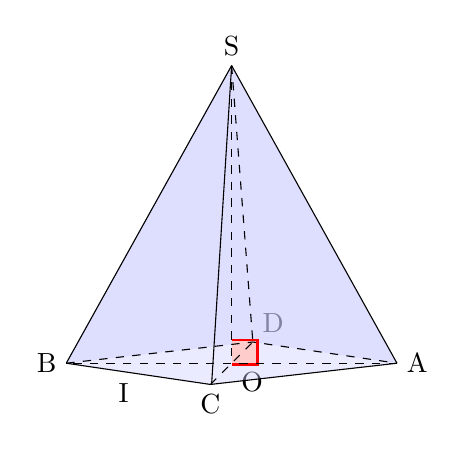
\begin{tikzpicture}[x=3cm,y=1.8cm,scale=0.7]
\tikzstyle{conefill} = [fill=blue!20,fill opacity=0.4] %couleur de fond
   
%coordonnées des sommets
\draw(0,3,0)node[above](S){S};
\draw(1,0,0)node[right](A){A};
\draw(-1,0,0)node[left](B){B};
\draw(0,0,1)node[below](C){C};
\draw(0,0,-1)node[above right](D){D};
\draw(0,0,0)node[below right](O){O};
\draw(-0.5,0,0.5)node[below left](I){I};

%remplir les faces
\fill[conefill] (1,0,0)--(0,0,1)--(1,0,0)--(0,0,-1)--cycle; %base
\fill[conefill] (0,3,0)--(-1,0,0)--(0,0,-1); %arrière gauche
\fill[conefill] (0,3,0)--(-1,0,0)--(0,0,1); %avant gauche
\fill[conefill] (0,3,0)--(0,0,1)--(1,0,0); %avant droit
\fill[conefill] (0,3,0)--(1,0,0)--(0,0,-1); %arrière droit

\draw [line width=2pt,color=red] (0,0,0)--(0.15,0,0)--(0.15,0.22,0)--(0,0.22,0);
\fill[color=red!20] (0,0,0)--(0.15,0,0)--(0.15,0.22,0)--(0,0.22,0);

%tracer les arêtes
\draw (A.west)--(C.north)--(B.east);
\draw[dashed] (B.east)--(D.south west)--(A.west);
\draw (S.south)--(A.west);
\draw (S.south)--(B.east);
\draw (S.south)--(C);
\draw[dashed] (S.south)--(D.south west);
   
\draw [dashed] (S)--(0,0,0);
\draw[dashed] (A)--(B);
\draw[dashed] (C.north)--(D.south west);  
\end{tikzpicture}


\item .

\vspace{-5.5cm}
\begin{flushright}

\includegraphics[scale=0.4]{../40.Image/DS5 - 1C.png}
\end{flushright}

\vspace{-4.5cm}
\item $OIS$ est un triangle rectangle en $O$ car $(OS)$ est la \\hauteur de la pyramide régulière $SABCD$

\item On sait que le triangle $OIS$ est rectangle en $O$.

\noindent On applique le théorème de Pythagore :

\vspace{-10mm}
\begin{eqnarray*}
IS^2 &=& OI^2 + OS^2 \\
&=& 7^2 + 24^2 \\
&=& 625\\
IS &=& \sqrt{625}\\
&=& 25
\end{eqnarray*}
La longueur du segment $IS$ est de $25$cm

\item Le patron de la pyramide est composé de $4$ triangles isocèles superposables et d'un carré.

\begin{minipage}[t]{8cm}
\noindent \textbf{Aire d'un carré :}

\vspace{-8mm}
\begin{eqnarray*}
\mathcal{A}_{carré} &=& c^2 \\
&=& BC^2 \\
&=& 14^2 \\
&=& 196
\end{eqnarray*}
\end{minipage}
\begin{minipage}[t]{8cm}
\noindent \textbf{Aire d'un triangle :}

\vspace{-8mm}
\begin{eqnarray*}
\mathcal{A}_{triangle} &=& \dfrac{b \times h}{2} \\
&=& \dfrac{BC \times SI}{2} \\
&=& \dfrac{14 \times 25}{2} \\
&=& 175
\end{eqnarray*}
\end{minipage}

\noindent \textbf{Aire de la pyramide}

\vspace{-8mm}
\begin{eqnarray*}
\mathcal{A}_{pyramide}&=& \mathcal{A}_{carré}  + 4 \times \mathcal{A}_{triangle} \\
&=& 196 + 4 \times 175 \\
&=& 896
\end{eqnarray*}
La surface de carton qui devra être allouer à la création de ce cône est de $896$cm$^2$
\end{enumerate}

\paragraph{Exercice 3}: \hfill \textbf{4 points}

\medskip\medskip
\noindent Masse de pommes de terre utilisé lors du record : \quad $6225$kg

\begin{center}
\renewcommand{\arraystretch}{2}
\begin{tabularx}{10cm}{|>{\columncolor{lightgray!50}}p{6cm}|*{2}{>{\centering \arraybackslash}X|}}
\hline
Masse de pomme de terre (en kg) & $622,5$ & $6225$ \\\hline
Volume de pomme de terre (en m$^3$) & $1$  & $V \quad ?$ \\\hline
\end{tabularx}
\end{center}

\medskip
\noindent Volume de pomme de terre utilisé lors du record : \quad $V \quad = \quad \dfrac{6225 \times 1}{622,5}$ \quad = \quad 10m$^3$

\medskip
\noindent Surface de la pyramide : \quad $S \quad = \quad \dfrac{3 \times V}{h} \quad = \quad \dfrac{3 \times 10}{7,5} \quad = \quad 4$m$^2$

\medskip
\noindent Coté de la pyramide : \quad $c \quad = \quad \sqrt{S} \quad = \quad \sqrt{4} \quad = \quad 2$m

\medskip
\noindent Le coté du cornet pour ce record du monde mesure $2$m 
\end{document}
